\documentclass[list, windows]{BHCexam}
\pagestyle{fancy}
\fancyfoot[C]{\kaishu \small 第 \thepage 页 共 \pageref{lastpage} 页}
\fancyhead[L]{
\includegraphics[width=2cm]{qrcode.png}}
\fancyhead[R]{\raisebox{0.5\height}{
\includegraphics[height=1cm]{logo.png}}}
\begin{document}
\title{上海某高中 2017-2018 学年度第一学期}
\subtitle{高一数学期中试卷}
\notice{满分150分,120分钟完成,允许使用计算器,答案一律写在答题纸上}
\author{微信关注公众号:橘子数学}
\date{2017.11}
\maketitle
\begin{groups}
\group{填空}{第1-6题每题4分,第7-12题每题5分.}

\begin{questions}[p]
\begin{minipage}{\linewidth}
\question [4] 已知集合$U=\{1,2,3,4\}$,集合$A=\{1,2\}$,$B=\{2,3\}$,则$(A\cap\complement_UB) \cup (\complement_UA\cap B)=$\key{$\{1,3\}$}.

\end{minipage}
\begin{solution}{4cm}
\method
$A\cap\complement_UB=\{1\}$, $B\cap\complement_UA=\{3\}$.

$(A\cap\complement_UB) \cup (\complement_UA\cap B)=\{1,3\}$.

\end{solution}
\vfill
\begin{minipage}{\linewidth}
\question [4] 设集合$M=\{x|0\lt x\leqslant{}3\}$,$N=\{x|0\lt x\leqslant{}2\}$,那么 “ $a\in{M}$ ” 是 “ $a\in{N}$ ” 的\key{必要非充分}条件.

\end{minipage}
\begin{solution}{4cm}
\method
由$N \subsetneqq M$,可知 “ $a\in{M}$ ” 是 “ $a\in{N}$ ” 的必要非充分条件.

\end{solution}
\vfill
\begin{minipage}{\linewidth}
\question [4] 函数$f(x)=\sqrt{x+1}+\dfrac{1}{2-x}$的定义域为\key{$[-1,2)\cup{}(2,+\infty)$}.

\end{minipage}
\begin{solution}{4cm}
\method
根据题意:$\left\{\begin{array}{l}{x+1\geqslant{}0}\\{2-x\neq{}0}\end{array}\right.$

解得:$x\geqslant{}-1$且$x\neq{}2$

定义域是:$[-1,2)\cup{}(2,+\infty)$.

\end{solution}
\vfill
\begin{minipage}{\linewidth}
\question [4] 已知集合$A=\{x \big| |x-a| \lt 1,x\in\symbf{R}\}$,
$B=\{x\Big|\dfrac{2x-a}{x+1} \lt 1,x\in\symbf{R}\}$,
且$A\cap B=\varnothing$,
 则实数$a$的取值范围是\key{$a \in (-\infty,-2]$}.

\end{minipage}
\begin{solution}{4cm}
\method
$A=(a-1,a+1)$,

由$\dfrac{2x-a}{x+1} \lt 1$化简得$\dfrac{x-a-1}{x+1} \lt 0$.

若$a+1 \gt -1$,不满足$A \cap B=\varnothing$.

若$a+1 \le -1$,满足$A \cap B=\varnothing$.

故$a\in(-\infty,-2]$.

\end{solution}
\vfill
\begin{minipage}{\linewidth}
\question [4] 已知$y=f(x), y=g(x)$是两个定义在$\symbf{R}$上的二次函数,其$x, y$的取值如下表所示: 
\[\begin{array}{|c|c|c|c|c|}
\hline
x & 1 & 2 & 3 & 4 \\
\hline
f(x) & -3 & -4 & -3 & 0\\
\hline
g(x) & 0 & 1 & 0 & -3\\
\hline
\end{array}\]
则不等式$f(g(x))\ge0$的解集为\key{$(-\infty,1]\cup[3,+\infty)$.}.

\end{minipage}
\begin{solution}{4cm}
\method
由表格可得$y=f(x)$图像开口向上且关于$x=2$对称,其零点为$x=4$和$x=0$.

故不等式$f(g(x))\ge0$, 即$g(x)\in(-\infty,0]\cup[4,+\infty)$.

又$y=g(x)$的图像开口向下且关于$x=2$对称,其最大值为$1$.

故$g(x)\in(-\infty,0]$,解得$x\in(-\infty,1]\cup[3,+\infty)$.

\end{solution}
\vfill
\begin{minipage}{\linewidth}
\question [4] 关于$x$的不等式$2kx^2+kx+\frac{3}{8} \lt 0$的解集不为空集,则$k$的取值范围为\key{$k \in (-\infty,0)\cup(3,+\infty)$}.

\end{minipage}
\begin{solution}{4cm}
\method
若$k \lt 0 $, 二次函数$y=2kx^2+kx+\frac{3}{8}$图像开口向下,解集恒不为空集. 满足.

若$k=0$, 不等式解集为$\varnothing$,不满足.

若$k \gt 0$,二次函数$y=2kx^2+kx+\frac{3}{8}$图像开口向上,要求$\Delta=k^2-4 \cdot (2k) \cdot \frac{3}{8}=k^2-3k \gt 0$,解得$k\in(3,+\infty)$.

综上所属,$k \in (-\infty,0)\cup(3,+\infty)$

\end{solution}
\vfill
\newpage
\begin{minipage}{\linewidth}
\question [5] 已知本张试卷的出卷人在公元$x^2$年时年龄为$x-8$岁,则出卷人的出生年份是\key{$1989$}.(假设出生当年的年龄为$1$岁)

\end{minipage}
\begin{solution}{4cm}
\method
设出卷人的出生年份是$y$.

则有$x^2-y+1=x-8$.

化简得$y=x^2-x+9$.

由生活常识,

$1952 \lt x^2-x+9 \lt 2000$, $x\in\symbf{N}$.

解得$x=45$, 故$y=1989$.

\end{solution}
\vfill
\begin{minipage}{\linewidth}
\question [5] 若对任意$x\in\symbf{R}$,不等式$|x|\geqslant{}ax$恒成立,则实数$a$的取值范围是\key{$a \in [-1,1]$}.

\end{minipage}
\begin{solution}{4cm}
\method
若$x \gt 0$,得$x \ge ax$, 解得$a \le 1$.

若$x = 0$,得$0 \ge 0$成立.

若$x \lt 0$,得$-x \ge ax$,解得$a \ge -1$.

综上所述,$a \in [-1,1]$.
\method
画出$y=|x|$与$y=ax$的图像, 

要使$y=ax$的图像恒在$y=|x|$下方,

则$a\in[-1,1]$.

\end{solution}
\vfill
\begin{minipage}{\linewidth}
\question [5] 设常数$a\gt \ 0$,若$9x+\dfrac{a^2}{x}\geqslant{}a+1$对一切正实数$x$成立,则$a$的取值范围为\key{$\left[\dfrac{1}{5}, + \infty \right)$}.

\end{minipage}
\begin{solution}{4cm}
\method
$\forall x\in{R}^{+},9x+\dfrac{a^2}{x}\geqslant{}2\sqrt{9x\cdot{}\dfrac{a^2}{x}}=6a$,

$\therefore{}6a\geqslant{}a+1$,

$\therefore{}a\geqslant{}\dfrac{1}{5}$.

\end{solution}
\vfill
\begin{minipage}{\linewidth}
\question [5] 设函数$f(x)=\begin{cases}x^2+2x+2,x\leqslant{}0\\-x^2,x\gt \ 0\end{cases}$,若$f(f(a))=2$,则$a=$\key{}.

\end{minipage}
\begin{solution}{4cm}
\method
若$a\leqslant{}0$, 
则$f(a)=a^2+2a+2=(a+1)^2+1 \gt 0$, 
而$f(f(a))=-(a^2+2a+2)^2=2$无解,舍去;

若$a\gt \ 0$,
则$f(a)=-a^2\lt 0$,
故$f(f(a))=(-a^2)^2+2(-a^2)+2=2$,
解得$a=\sqrt{2}$.

综上所述, $a=\sqrt{2}$.

\end{solution}
\vfill
\begin{minipage}{\linewidth}
\question [5] 若二次函数$y=f(x)$对一切$x\in \text{R}$恒有${{x}^{2}}-2x+4\le f(x)\le 2{{x}^{2}}-4x+5$成立,且$f(5)=27$,则$f(11)=$\key{$153$}.

\end{minipage}
\begin{solution}{4cm}
\method
画出不等式两边的两个二次函数图像,如图,可得未知的二次函数$y=f(x)$开口向上,以$(1,3)$为顶点,故可设函数解析式为$f(x)=a(x-1)^2+3$,将$f(5)=27$代入可得$a=\frac{3}{2}$,则$f(x)=\frac{3}{2}(x-1)^2+3$,故$f(11)=153$.
\begin{center}
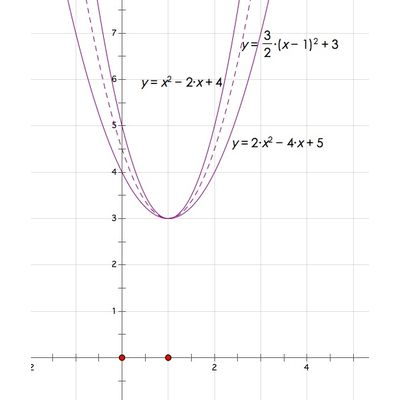
\includegraphics[height=8cm]{./To7VxKXpZaOWO5Qq9qzeZGtlwYTwJ5KF.jpg}\\
第11题
\vspace{0.5cm}
\end{center}

\end{solution}
\vfill
\begin{minipage}{\linewidth}
\question [5] 已知$f(x)=(a^2-5)x^2+2x+2$. 若不等式$f(x) \gt x$的解集为$A$. 已知$(0,1)\subseteq A$,则$a$的取值范围为\key{$a \in (-\infty,-\sqrt{2}]\cup[\sqrt{2},+\infty)$}.

\end{minipage}
\begin{solution}{4cm}
\method
由题意得,$(a^2-5)x^2+x+2 \gt 0$在$(0,1)$上恒成立.

即$a^2-5 \gt -\frac{2}{x^2}-\frac{1}{x}$在$(0,1)$上恒成立.

设$f(x)=-\frac{2}{x^2}-\frac{1}{x}=-2(\frac{1}{x}+\frac{1}{4})^2+\frac{1}{8}$, 

又$\frac{1}{x}\in(1,+\infty)$, 故$f(x) \lt -3$.

即$a^2-5 \ge -3$, 解得$a \in (-\infty,-\sqrt{2}]\cup[\sqrt{2},+\infty)$.

\end{solution}
\end{questions}

\group{选择}{第13-16题每题5分.}

\begin{questions}[p]
\begin{minipage}{\linewidth}
\question [5] 设$P,Q$为两个非空实数集,定义集合$P+Q=\{a+b|a\in{P},b\in{Q}\}$.若$P=\{0,2,5\}$,$Q=\{1,2,6\}$,则$P+Q$中元素的个数是\key{B}.
\fourchoices{$9$}{$8$}{$7$}{$6$}
\end{minipage}
\begin{solution}{4cm}
\method
$\because P=\{0,2,5\}$,$Q=\{1,2,6\}$,

$\therefore P+Q=\{1,2,3,4,6,7,8,11\}$.

故选B

\end{solution}
\vfill
\begin{minipage}{\linewidth}
\question [5] 不等式$(1+x)(1-|x|)\gt \ 0$的解集是\key{D}.
\fourchoices{$\{x|0\leqslant{}x\lt 1\}$}{$\{x|x\lt 0$且$x\neq{}-1\}$}{$\{x|-1\lt x\lt 1\}$}{$\{x|x\lt 1$且$x\neq{}-1\}$}
\end{minipage}
\begin{solution}{4cm}
\method
求不等式$(1+x)(1-|x|)\gt \ 0$的解集,则分两种情况讨论:

情况$1:\left\{\begin{array}{l}{1+x\gt \ 0\;\;}\\{1-|x|\gt \ 0}\end{array}\right.$

即$\left\{\begin{array}{l}{x\gt \ -1}\\{-1\lt x\lt 1}\end{array}\right.$
则$-1\lt x\lt 1$.

情况$2:\left\{\begin{array}{l}{1+x\lt 0}\\{1-|x|\lt 0}\end{array}\right.$

即$\left\{\begin{array}{l}{x\lt -1}\\{x\gt 1\text{或}x\lt -1}\end{array}\right.$
则$x\lt -1$.

两种情况取并集得$\{x|x\lt 1$且$x\neq{}-1\}$.

故选D.

\end{solution}
\vfill
\begin{minipage}{\linewidth}
\question [5] 已知三个不等式:$ab\gt \ 0$,$bc-ad\gt \ 0$,$\dfrac{c}{a}-\dfrac{d}{b}\gt \ 0$(其中$a,b,c,d$均为实数),用其中两个不等式作为条件,余下的一个不等式作为结论组成一个命题,可组成的正确命题的个数是\key{D}.
\fourchoices{$0$}{$1$}{$2$}{$3$}
\end{minipage}
\begin{solution}{4cm}
\method
$\begin{cases}ab\gt \ 0, &\cdots(1)\\
bc-ad\gt \ 0,&\cdots(2)
\end{cases}$

$(2)\div(1)$得$\dfrac{bc-ad}{ab}=\dfrac{c}{a}-\dfrac{d}{b}\gt \ 0$.

$\begin{cases}
ab\gt \ 0,&\cdots(1)\\
\dfrac{c}{a}-\dfrac{d}{b}\gt \ 0,&\cdots(3)
\end{cases}$

$(1)\times{}(3)$得$ab(\dfrac{c}{a}-\dfrac{d}{b})=bc-ad\gt \ 0$.

$\begin{cases}bc-ad\gt \ 0,&\cdots(2)\\
\dfrac{c}{a}-\dfrac{d}{b}\gt \ 0,&\cdots(3)
\end{cases}$

用反证法,显然$ab\neq{}0$,

设$ab\lt 0$,$(2)$式同除$ab$得$\dfrac{c}{a}-\dfrac{d}{b}\lt 0$,矛盾,

故$ab\gt \ 0$.
故选D.

\end{solution}
\vfill
\begin{minipage}{\linewidth}
\question [5] 设$a\gt \ 0$,$b\gt \ 0$,则以下不等式中不恒成立的是\key{B}.
\fourchoices{$(a+b)(\dfrac{1}{a}+\dfrac{1}{b})\geqslant{}4$}{$a^{3}+b^{3}\geqslant{}2ab^{2}$}{$a^{2}+b^{2}+2\geqslant{}2a+2b$}{$\sqrt{|{a-b}|}\geqslant{}\sqrt{a}-\sqrt{b}$}
\end{minipage}
\begin{solution}{4cm}
\method
$a\gt \ 0$,$b\gt \ 0$,

$(a+b)(\dfrac{1}{a}+\dfrac{1}{b})\geqslant{}2\sqrt{ab}\cdot{}2\sqrt{\dfrac{1}{ab}}\geqslant{}4$,

故A恒成立;

$a^{3}+b^{3}\geqslant{}2ab^{2}$,

取$a=\dfrac{1}{2}$,$b=\dfrac{2}{3}$,则B不成立;

$a^{2}+b^{2}+2-(2a+2b)=(a-1)^{2}+(b-1)^{2}\geqslant{}0$,

故C恒成立;

若$a\lt b$,则$\sqrt{|{a-b}|}\geqslant{}\sqrt{a}-\sqrt{b}$恒成立,

若$a\geqslant{}b$,则${(\sqrt{|{a-b}|})^2}-{(\sqrt{a}-\sqrt{b})^2}=2\sqrt{ab}\geqslant{}0$,

故$\sqrt{|{a-b}|}\geqslant{}\sqrt{a}-\sqrt{b}$,
即D恒成立.

\end{solution}
\end{questions}
\group{简答}{第17-19题每题14分,第20题16分,第21题18分.}

\begin{questions}[stp]
\begin{minipage}{\linewidth}
\question [14] 已知$\triangle ABC$为直角三角形, 记其两条直角边长分别为$a,b\in\symbf{R}^+$, 记面积为$S$, 周长为$C$. 若三角形面积为定值,其周长是否有最值,最大值还是最小值,何时取到,为多少(结果用$S$表示)?

\end{minipage}
\begin{solution}{6cm}
\method
$C=a+b+\sqrt{a^2+b^2}$,
\score{2}{2}由$\sqrt{a^2+b^2} \ge \sqrt{2ab}$,$a+b \ge 2\sqrt{ab}$,

得$C \ge  2\sqrt{ab}+\sqrt{2ab}$
\score{6}{8}由$S=\frac{1}{2}ab$,

得$C \ge (2+2\sqrt{2})\sqrt{S}$,
\score{4}{12}当且仅当$a=b=\sqrt{2S}$时取到最小值.
\score{2}{14}
\end{solution}
\vfill
\begin{minipage}{\linewidth}
\question [14] 已知$a\in\textbf{R}$,若关于$x$的方程$x^2+x+|a-\dfrac{1}{4}|+|a|=0$有实根,求$a$的取值范围.

\end{minipage}
\begin{solution}{6cm}
\method
方程即$|a-\frac{1}{4}|+|a|=-x^2-x\in[0,\frac{1}{4}]$,

即解不等式$|a-\frac{1}{4}|+|a| \le \frac{1}{4}$.

当$a\le 0$,化简得$\frac{1}{4}-2a \le \frac{1}{4}$,解得$a=0$;

当$0 \lt a\le \frac{1}{4}$, 化简得$\frac{1}{4} \le \frac{1}{4}$,解得$a\in(0,\frac{1}{4}]$;

当$a \gt \frac{1}{4}$, 化简得$2a-\frac{1}{4}\le\frac{1}{4}$,无解.

综上所述,$a\in [0,\frac{1}{4}]$
\score{14}{14}
\end{solution}
\vfill
\newpage
\begin{minipage}{\linewidth}
\question [14] 先阅读下列不等式的证法,再解决后面的问题:
\[
\text{证明:} (a_1b_1+a_2b_2)^2 \le  (a_1^2+a_2^2)(b_1^2+b_2^2)\]

证: 令$A=\sqrt{a_1^2+a_2^2}$, $B=\sqrt{b_1^2+b_2^2}$

\[
\begin{array}{rl}
\frac{a_1b_1+a_2b_2}{\sqrt{a_1^2+a_2^2}\sqrt{b_1^2+b_2^2}}& =\frac{a_1b_1}{AB}+\frac{a_2b_2}{AB}\\
& = \frac{a_1}{A}\cdot\frac{b_1}{B}+\frac{a_2}{A}\cdot\frac{b_2}{B} \\
& \le \frac{1}{2}(\frac{a_1^2}{A^2}+\frac{b_1^2}{B^2})+ \frac{1}{2}(\frac{a_2^2}{A^2}+\frac{b_2^2}{B^2})\\
& =\frac{1}{2}(\frac{a_1^2+a_2^2}{A^2}+\frac{b_1^2+b_2^2}{B^2})\\
& =1
\end{array}
\]
故$ (a_1b_1+a_2b_2)^2 \le  (a_1^2+a_2^2)(b_1^2+b_2^2)$.
\begin{subquestions}
    \subquestion 若$x_1,y_1,x_2,y_2\in\symbf{R^+}$,利用上述结论,证明:\[
(x_1+x_2)(y_1+y_2) \ge (\sqrt{x_1y_1}+\sqrt{x_2y_2})^2
\]
    \subquestion 若$x_1,y_1,x_2,y_2,z_1,z_2\in\symbf{R^+}$,模仿上述证法并结合(1)的证法,证明:\[
(x_1+x_2)(y_1+y_2)(z_1+z_2) \ge (\sqrt[3]{x_1y_1z_1}+\sqrt[3]{x_2y_2z_2})^3
\]
(提示:若$a,b,c\in\symbf{R^+}$,有$\frac{a^3+b^3+c^3}{3}\ge abc$,)
\end{subquestions}
\end{minipage}
\begin{solution}{3cm}
\method
(1)设$a_1=\sqrt{x_1}$,$a_2=\sqrt{x_2}$,$b_1=\sqrt{y_1}$,$b_2=\sqrt{y_2}$.

由\[ (a_1b_1+a_2b_2)^2 \le  (a_1^2+a_2^2)(b_1^2+b_2^2)\]

得\[ (\sqrt{x_1}\sqrt{y_1}+\sqrt{x_2}\sqrt{y_2})^2 \le  [((\sqrt{x_1})^2+(\sqrt{x_2})^2)((\sqrt{y_1})^2+(\sqrt{y_2})^2)]\]

即\[
(x_1+x_2)(y_1+y_2) \ge (\sqrt{x_1y_1}+\sqrt{x_2y_2})^2
\]
\score{6}{6}(2) 设$a_1=\sqrt[3]{x_1}, b_1=\sqrt[3]{y_1}, c_1=\sqrt[3]{z_1}$, $a_2=\sqrt[3]{x_2}, b_2=\sqrt[3]{y_2}, c_2=\sqrt[3]{z_2}$.

要证
\[
(x_1+x_2)(y_1+y_2)(z_1+z_2) \ge (\sqrt[3]{x_1y_1z_1}+\sqrt[3]{x_2y_2z_2})^3
\]

即证
\[
(a_1b_1c_1+a_2b_2c_2)^3 \le  (a_1^3+a_2^3)(b_1^3+b_2^3)(c_1^3+c_2^3)
\]

(不换元,直接证不扣分)
\score{2}{8}令$A=\sqrt[3]{a_1^3+a_2^3}$,$B=\sqrt[3]{b_1^3+b_2^3}$, $C=\sqrt[3]{c_1^3+c_2^3}$.

\[
\begin{array}{rl}
& \frac{a_1b_1c_1+a_2b_2c_2}{\sqrt[3]{a_1^3+a_2^3}\sqrt[3]{b_1^3+b_2^3}\sqrt[3]{c_1^3+c_2^3}}\\
= & \frac{a_1b_1c_1}{ABC}+\frac{a_2b_2c_2}{ABC}\\
= & \frac{a_1}{A}\cdot\frac{b_1}{B}\cdot\frac{c_1}{C}+\frac{a_2}{A}\cdot\frac{b_2}{B}\cdot\frac{c_2}{C}\\
\le & \frac{1}{3}(\frac{a_1^3}{A^3}+\frac{b_1^3}{B^3}+\frac{c_1^3}{C^3})+ \frac{1}{3}(\frac{a_2^3}{A^3}+\frac{b_2^3}{B^3}+\frac{c_2^3}{C^3})\\
= & \frac{1}{3}(\frac{a_1^3+a_2^3}{A^3}+\frac{b_1^3+b_2^3}{B^3}++\frac{c_1^3+c_2^3}{C^3})\\
= & 1
\end{array}
\]

故\[(a_1b_1c_1+a_2b_2c_2)^3 \le  (a_1^3+a_2^3)(b_1^3+b_2^3)(c_1^3+c_2^3)\]

得证.
\score{6}{14}
\end{solution}
\vfill
\newpage
\begin{minipage}{\linewidth}
\question [16] 公元2222年,有一种高危传染疾病在全球范围内蔓延,被感染者的潜伏期可以长达10年,期间会有约$0.05\%$的概率传染给他人,一旦发病三天内即死亡。某城市总人口约200万人,专家分析其中约有$1000$名感染者,为了防止疾病继续扩散,疾病预防控制中心现决定对全市人口进行血液检测以筛选出被感染者。由于检测试剂十分昂贵且数量有限,需要将血样混合后一起检测以节约试剂。已知感染者的检测结果为阳性, 未被感染者则为阴性. 阳性血样与阴性血样混合后的检测结果为阳性, 同为阴性或阳性的血样混合后结果不发生改变.
\begin{subquestions}
    \subquestion 若对全市人口进行平均分组,同一分组的血样将被混合到一起检测,若发现结果为阳性,则再在该分组内逐个检测排查. 设每个组$x$个人,那么最坏情况下,需要进行约多少次检测可以找到所有的被感染者? 在当前方案下,若要使检测的次数尽可能少,每个分组的最优人数是?
    \subquestion 在(1)的检测方案中,对于检测结果为阳性的组采取逐一检测排查的方法并不是很好,或可将这些组的血样再进行一次分组混合血样检测,然后再进行逐一排查。仍然考虑最坏的情况,请问两次要如何分组,使检测总次数尽可能少?
    \subquestion 在(2)的检测方案中,进行了两次分组混合血样检测。仍然考虑最坏情况,若再进行若干次分组混合血样检测,是否会使检测次数更少?请给出最优的检测方案.
\end{subquestions}
\end{minipage}
\begin{solution}{6cm}
\method
设需要进行$y$次检测. 由每个组$x$个人,则有$\frac{2000000}{x}$个小组, 最坏情况是1000人被分配到了不同的组. 

\[
y=\begin{cases}
\frac{2\cdot 10^6}{x}+2\cdot 10^6, & x \ge 2000 \\
\frac{2\cdot 10^6}{x}+1000\cdot x, & x \lt 2000 \\
\end{cases}
\]

(题目要求近似计算,可以不考虑整除,考虑整除不扣分)
\score{2}{2}分组数小于1000的情况比逐个检测还要多,可以不用考虑,

$y=\frac{2\times 10^6}{x}+1000\cdot x \ge 2\sqrt{2\cdot 10^9}$.

当$x=\sqrt{2\times10^3}\approx45$人,检测次数最少.

(结果为44-45都给分)
\score{2}{4}(2) 设第二次分组每个组$w$人.

\[
\begin{array}{rl}
y & = \frac{2\times10^6}{x}+\frac{1000x}{w}+1000w\\
& \ge 3\sqrt[3]{2\times10^{12}}\\
\end{array}
\]

当$\frac{2\times10^6}{x}=\frac{1000x}{w}=1000w$时,
即$x=2000^\frac{2}{3}\approx159$,$w=2000^\frac{1}{3}\approx13$,
检测次数最少.

所以第一次分组159人一组,第二次分组13人一组.

(也可以用两次基本不等式求得,允许$10\%$的误差.)
\score{6}{10}(3) 若进行$k$次分组,设第$i$次分组时每组人数为$x_i$. 则总的检测次数为:
\[
\begin{array}{rl}
y=&\dfrac{2\times10^6}{x_1}+\dfrac{1000x_1}{x_2}+\cdots\\
&+\dfrac{1000x_{k-1}}{x_k}+1000x_k\\
\ge & (k+1)\sqrt[k+1]{2\times10^{3k+2}}
\end{array}
\]

利用计算器可得,

1次分组, $y \ge 2\sqrt{2\cdot 10^9}\approx8.94\times10^4$;

2次分组, $y \ge 3\sqrt[3]{2\cdot 10^{12}}\approx3.78\times10^4$;

3次分组, $y \ge 4\sqrt[4]{2\cdot 10^{15}}\approx2.68\times10^4$;

4次分组, $y \ge 5\sqrt[5]{2\cdot 10^{18}}\approx2.29\times10^4$;

5次分组, $y \ge 6\sqrt[6]{2\cdot 10^{21}}\approx2.13\times10^4$;

6次分组, $y \ge 7\sqrt[7]{2\cdot 10^{24}}\approx2.073\times10^4$;

7次分组, $y \ge 8\sqrt[8]{2\cdot 10^{27}}\approx2.068\times10^4$;

8次分组, $y \ge 9\sqrt[9]{2\cdot 10^{30}}\approx2.094\times10^4$;

9次分组, $y \ge 10\sqrt[10]{2\cdot 10^{33}}\approx2.138\times10^4$;

可见进行7次分组混合血样检测最优.

其中第k次分组时$(2000)^{\frac{8-k}{8}}$人一组.
\score{6}{16}
\end{solution}
\vfill
\newpage
\begin{minipage}{\linewidth}
\question [18] 已知函数$f(x)=a{{x}^{2}}-\frac{1}{2}x+c$($a$、$c\in R$),满足$f(1)=0$,且$f(x)\ge 0$在$x\in R$时恒成立.
\begin{subquestions}
    \subquestion 求$a$、$c$的值;
    \subquestion 若$h(x)=\frac{3}{4}{{x}^{2}}-bx+\frac{b}{2}-\frac{1}{4}$,解不等式$f(x)+h(x) \lt 0$;
    \subquestion 是否存在实数$m$,使函数$g(x)=f(x)-mx$在区间$[m,m+2]$上有最小值$-5$?若存在,请求出$m$的值;若不存在,请说明理由.
\end{subquestions}
\end{minipage}
\begin{solution}{6cm}
\method
由$f(1)=0$,得$a+c=\frac{1}{2}$,
\score{1}{1}因为$f(x)\ge 0$在$x\in R$时恒成立,所以$a \gt 0$且△$=\frac{1}{4}-4ac\le 0$,$ac\ge \frac{1}{16}$,
\score{1}{2}即$a\left( \frac{1}{2}-a \right)\ge \frac{1}{16}$,${{a}^{2}}-\frac{1}{2}a+\frac{1}{16}\le 0$,${{\left( a-\frac{1}{4} \right)}^{2}}\le 0$,所以$a=c=\frac{1}{4}$.
\score{2}{4}(2) 由(1)得$f(x)=\frac{1}{4}{{x}^{2}}-\frac{1}{2}x+\frac{1}{4}$,由$f(x)+h(x) \lt 0$,得
${{x}^{2}}-\left( b+\frac{1}{2} \right)x+\frac{b}{2} \lt 0$,即$(x-b)\left( x-\frac{1}{2} \right) \lt 0$,
\score{3}{7}所以,当$b \lt \frac{1}{2}$时,原不等式解集为$(b,\frac{1}{2})$;
当$b \gt \frac{1}{2}$时,原不等式解集为$(\frac{1}{2},b)$;
当$b=\frac{1}{2}$时,原不等式解集为空集 .
\score{3}{10}(3) $g(x)=\frac{1}{4}{{x}^{2}}-\left( \frac{1}{2}+m \right)x+\frac{1}{4}$,
\score{1}{11}$g(x)$的图像是开口向上的抛物线,对称轴为直线$x=2m+1$.
假设存在实数$m$,使函数$g(x)$在区间$[m,m+2]$上有最小值$-5$.
\ding{192}	当$2m+1 \lt m$,即$m \lt -1$时,函数$g(x)$在区间$[m,m+2]$上是增函数,所以$g(m)=-5$,即$\frac{1}{4}{{m}^{2}}-\left( \frac{1}{2}+m \right)m+\frac{1}{4}=-5$,解得$m=-3$或$m=\frac{7}{3}$,
因为$m \lt -1$,所以$m=-3$;
\score{2}{13}\ding{193}当$m\le 2m+1\le m+2$,即$-1\le m\le 1$时,函数$g(x)$的最小值为$g(2m+1)=-5$,即
$\frac{1}{4}{{(2m+1)}^{2}}-\left( \frac{1}{2}+m \right)(2m+1)+\frac{1}{4}=-5$,解得$m=-\frac{1}{2}-\frac{\sqrt{21}}{2}$或$m=-\frac{1}{2}+\frac{\sqrt{21}}{2}$,均舍去;
\score{2}{15}\ding{194}当$2m+1 \gt m+2$,即$m \gt 1$时,$g(x)$在区间$[m,m+2]$上是减函数,所以$g(m+2)=-5$,即$\frac{1}{4}{{(m+2)}^{2}}-\left( \frac{1}{2}+m \right)(m+2)+\frac{1}{4}=-5$,解得$m=-1-2\sqrt{2}$或$m=-1+2\sqrt{2}$,因$m \gt 1$,所以$m=-1+2\sqrt{2}$.
\score{2}{17}综上,存在实数$m$,$m=-3$或$m=-1+2\sqrt{2}$时,函数$g(x)$在区间$[m,m+2]$上有最小值$-5$.
\score{1}{18}
\end{solution}
\end{questions}
\end{groups}
\label{lastpage}
\end{document}
